\chapter{Katnabour}
\label{ch:katnabour}
\index{dessert}
\index{rice}
\index{pudding}

\marginnote{
    \textbf{Makes 1 bowl} \\
    Prep time: 5 minutes \\
    Cook time: 30 minutes \\
    \vspace*{\baselineskip}

    1/2 cup rice, Calrose \\
    3 cups milk, 2\% \\
    3 tbsp sugar 
}

\textit{Rice pudding}

Family member: Sybil

\newthought{Secret tip:} microwave for a few second and serve warm in a small coffee cup with a sprinkle of cinnamon.

\begin{marginfigure}
  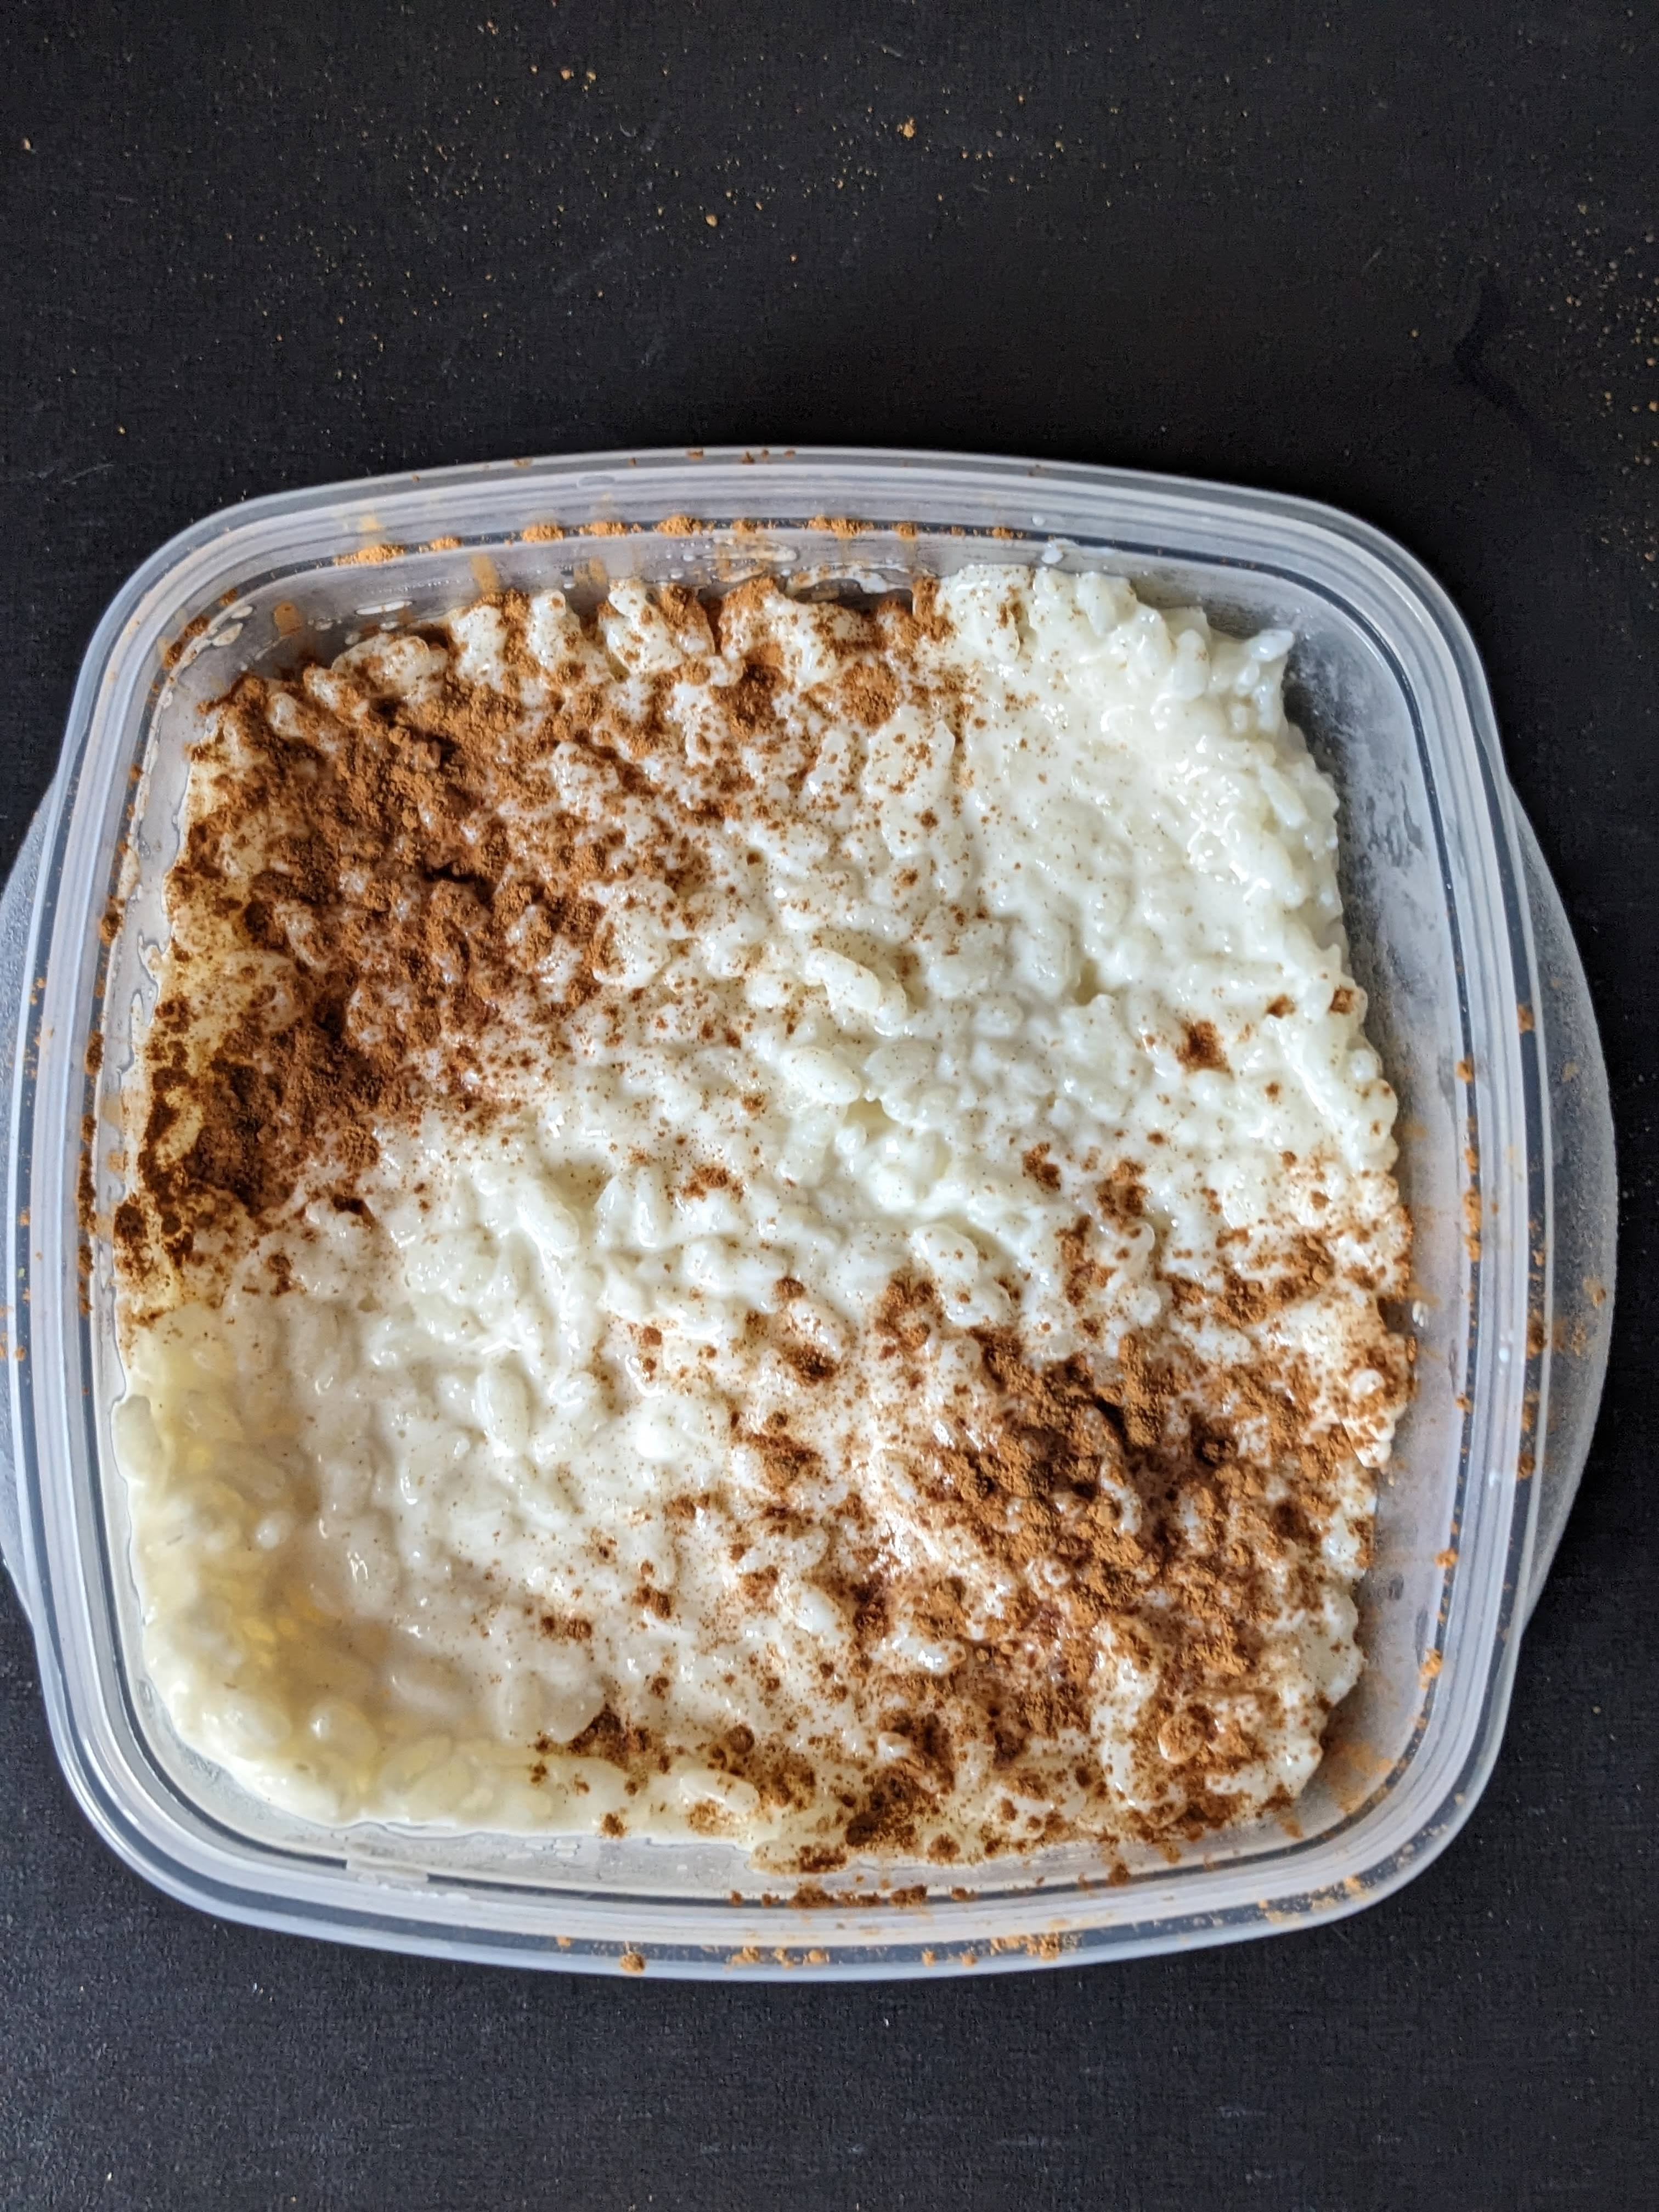
\includegraphics[width=60mm]{dermardiros/images/Rice pudding.jpg}
  \caption{Anoushabour made in Barcelona}
\end{marginfigure}


\begin{enumerate}
    \item In a pot, cook the rice in 1 cup of milk on low heat.
    \item Gradually add 1 cup of milk at a time, once milk has been absorbed.
    \item When all the milk has been added and the rice is cooked, add the sugar. 
    \item Cook on low heat for maximum 5 minutes then set the pot aside to cool.
\end{enumerate}
